\newif\ifexternalize
\externalizetrue

\documentclass{article}
\usepackage{pgfplots}
\newcommand{\figurefilename}[1]{\ifexternalize \tikzsetnextfilename{#1} \fi}
\ifexternalize															%
	\usetikzlibrary{external}											%
	\tikzexternalize[shell escape=-enable-write18]						%
	\tikzset{external/force remake}										%
\fi																		%



\begin{document}

\figurefilenam{figure-blabla}
\begin{figure}[!htbp]
	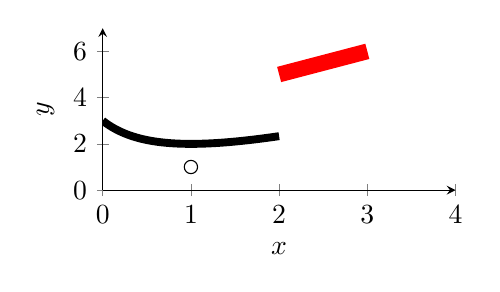
\begin{tikzpicture}
		%
		\begin{axis}
		[
			xmode					= linear,
			ymode					= linear,
			width					= 0.5\columnwidth,
			height					= 0.3\columnwidth,
			axis x line				= bottom,	% bottom | middle | top
			axis y line				= left,		% left | middle | right
			xlabel					= {$x$},
			ylabel					= {$y$},
			xmin					= 0,
			xmax					= 4,
			ymin					= 0,
			ymax					= 7,
		]
			%
			\addplot
			[
				no marks,
				smooth,
				domain	= 0:2,
				samples = 100,
				black,
				line width = 0.1cm,
			]
			{(x^2 + 3)/(x + 1)};
			%
			\addplot
			[
				no marks,
				smooth,
				domain	= 2:3,
				samples = 100,
				red,
				line width = 0.2cm,
			]
			{x + 3};
			%
			% ALLOWED OPERATORS
			% +, -, *, /, abs, round, floor, mod, <, >, max, min, sin, cos, tan,
			% deg (conversion from radians to degrees),
			% rad (conversion from degrees to radians),
			% atan, asin, acos, cot, sec, cosec, exp, ln,
			% sqrt, the constants pi and e, ^ (power operation), factorial,
			% rand (random between −1 and 1), rnd (random between 0 and 1),
			% number format conversions hex, Hex, oct, bin
			%
			\addplot
			[
				scatter,
				scatter/use mapped color = {black},
				only marks,
				mark options	=
				{
					scale 		= 1.2,
					draw		= black,
					fill		= white,
					opacity		= 1.0
				},
				mark			= o, % other options (may require \usetikzlibrary{plotmarks}): pentagon | pentagon* | text | cube | cube* | + | − | | | o | asterisk | star | 10-pointed star | oplus | oplus* | otimes | otimes* | square | square* | triangle | triangle* | diamond | diamond* | halfdiamond* | halfsquare* | halfsquare right* | halfsquare left* | Mercedes star | Mercedes star flipped | halfcircle | halfcircle* 
			]
			coordinates {(1,1)};
			%
		\end{axis}
		%
	\end{tikzpicture}
\end{figure}

\end{document}
